
\subsubsection{Cross over gadget}

The idea this gadget is to assemble after reading the MSD, routing the counter back to the start of the
next row, in position for the counter to begin reading the first digit.
The number of tiles shaded in darker grey is $6 \cdot \floor*{\frac{d}{3}}$.

\vspace{.5cm}
For each $\inc\in \{ {\tt increment}, {\tt copy} \}$:

\begin{itemize}
    \item Create
    $\begin{aligned}[t]
        {\tt Cross\_Next\_Row}(&\left\langle {\tt CrossNextRow},            \inc \right\rangle,
                                \left\langle {\tt CounterRead},        1, \lambda, \inc \right\rangle \;)
    \end{aligned}$\\from the gadget shown in Figure~\ref{fig:cross_next_row}.
\end{itemize}


\begin{figure}[H]
    \centering
    \subcaptionbox{
        General.
        \label{fig:cross_next_row}
    }{\makebox[0.24\textwidth][c]{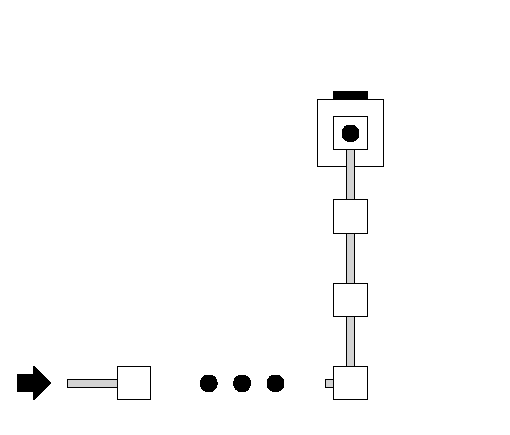
\includegraphics[width=1in]{cross_next_row}}}%
    ~
    \subcaptionbox{
        General overview.
        The black tiles in this figure is the gadget shown in subfigure~\subref{fig:cross_next_row}.
        \label{fig:cross_next_row_overview}
    }{\makebox[0.30\textwidth][c]{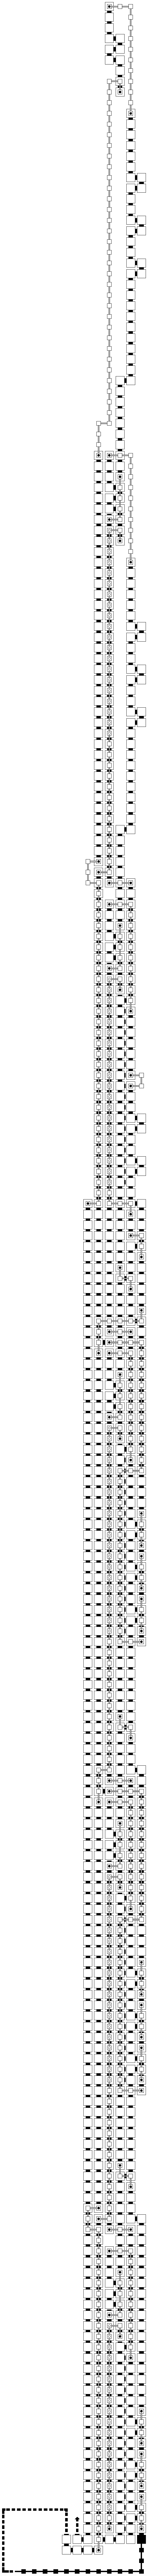
\includegraphics[width=0.45in]{overviews/general/crosser}}}%
    ~
    \caption{\label{fig:crosser_gadgets} The {\tt Cross\_Next\_Row} gadget.}
\end{figure}
